\section{原型系统设计}
\label{chap:linphone:designation}

本节主要介绍Linphone环境下,时间隐通道原型系统的模块设计,及模块之间的关联与数据流。

\subsection{设计架构及模块关联}
\label{chap:linphone:designation:struct}

\insertFigure{
	\begin{figure}[htbp]
		\centering
        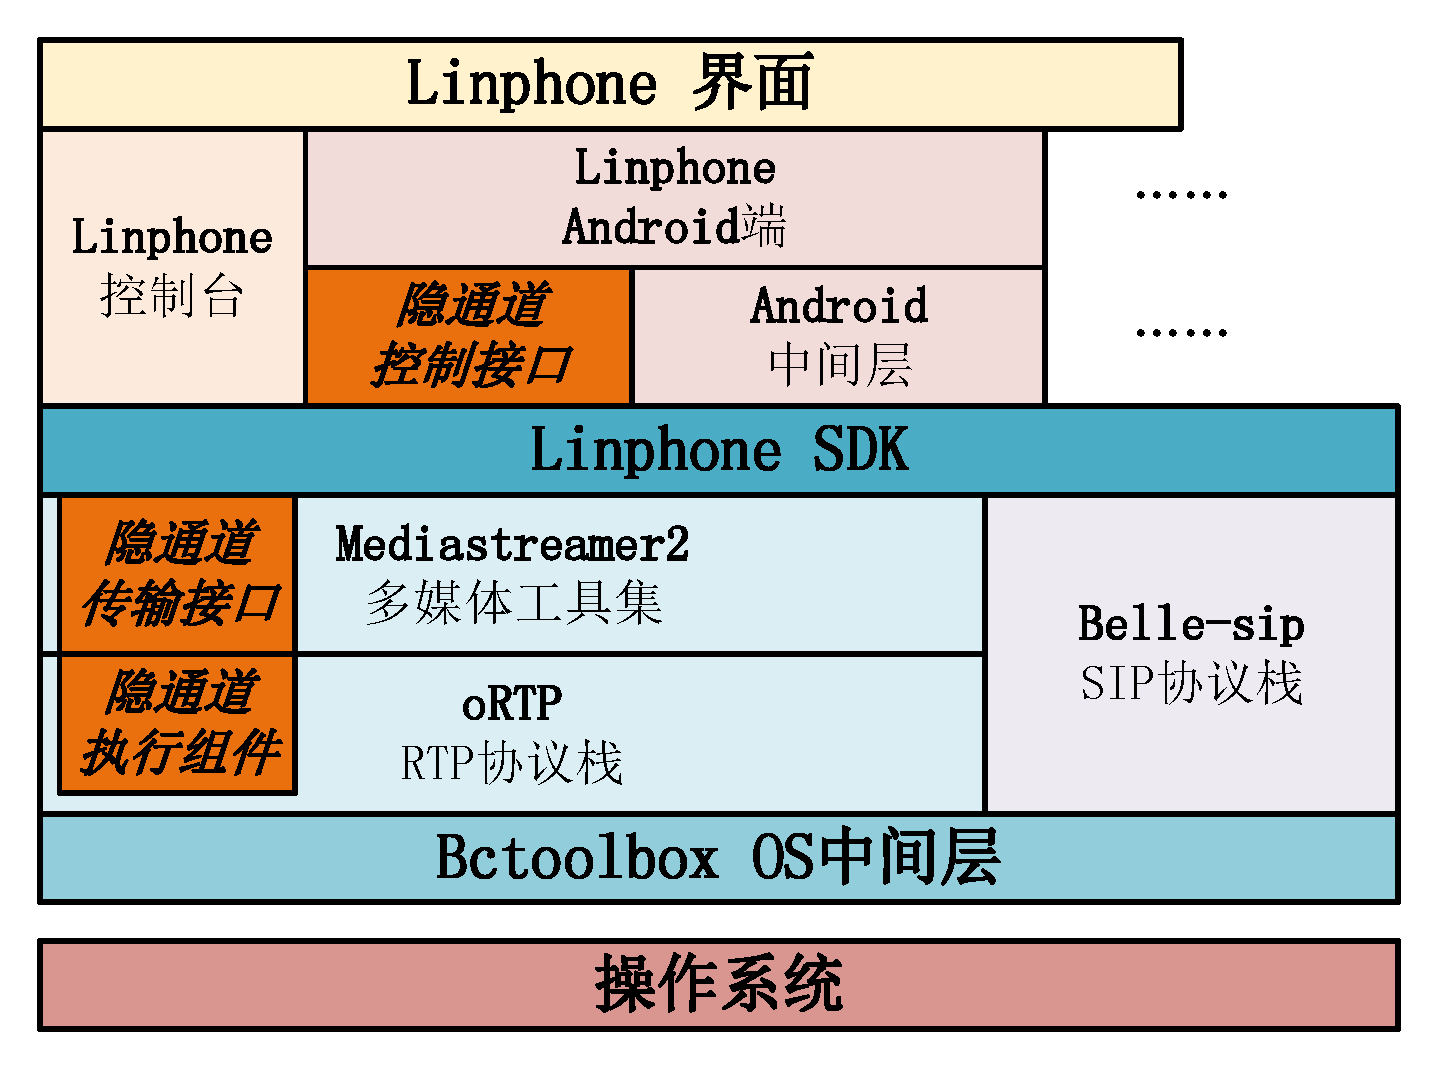
\includegraphics[width=0.65\textwidth]{chapters/chapter6/figures/ctc-struct.pdf}
        \caption{原型系统的模块分布图}
        \label{fig:6:ctc-struct}
    \end{figure}
}

如图\ \nref{fig:6:ctc-struct},原型系统的模块包括三部分,分别为隐通道控制接口、隐通道消息接口及隐通道执行组件。其中,隐通道控制接口位于Linphone Android端的界面层,负责接收用户的控制命令,并反馈响应结果。隐通道消息接口位于Mediastreamer2层,负责隐通道控制接口及隐通道执行组件之间的数据及控制流传输。隐通道执行组件位于oRTP层,负责控制与监听RTP数据包传输,以及实现时间隐通道传输逻辑。

\subsection{用户控制接口设计}
\label{chap:linphone:designation:ui}

\insertFigure{
	\begin{figure}[htb]
		\centering
        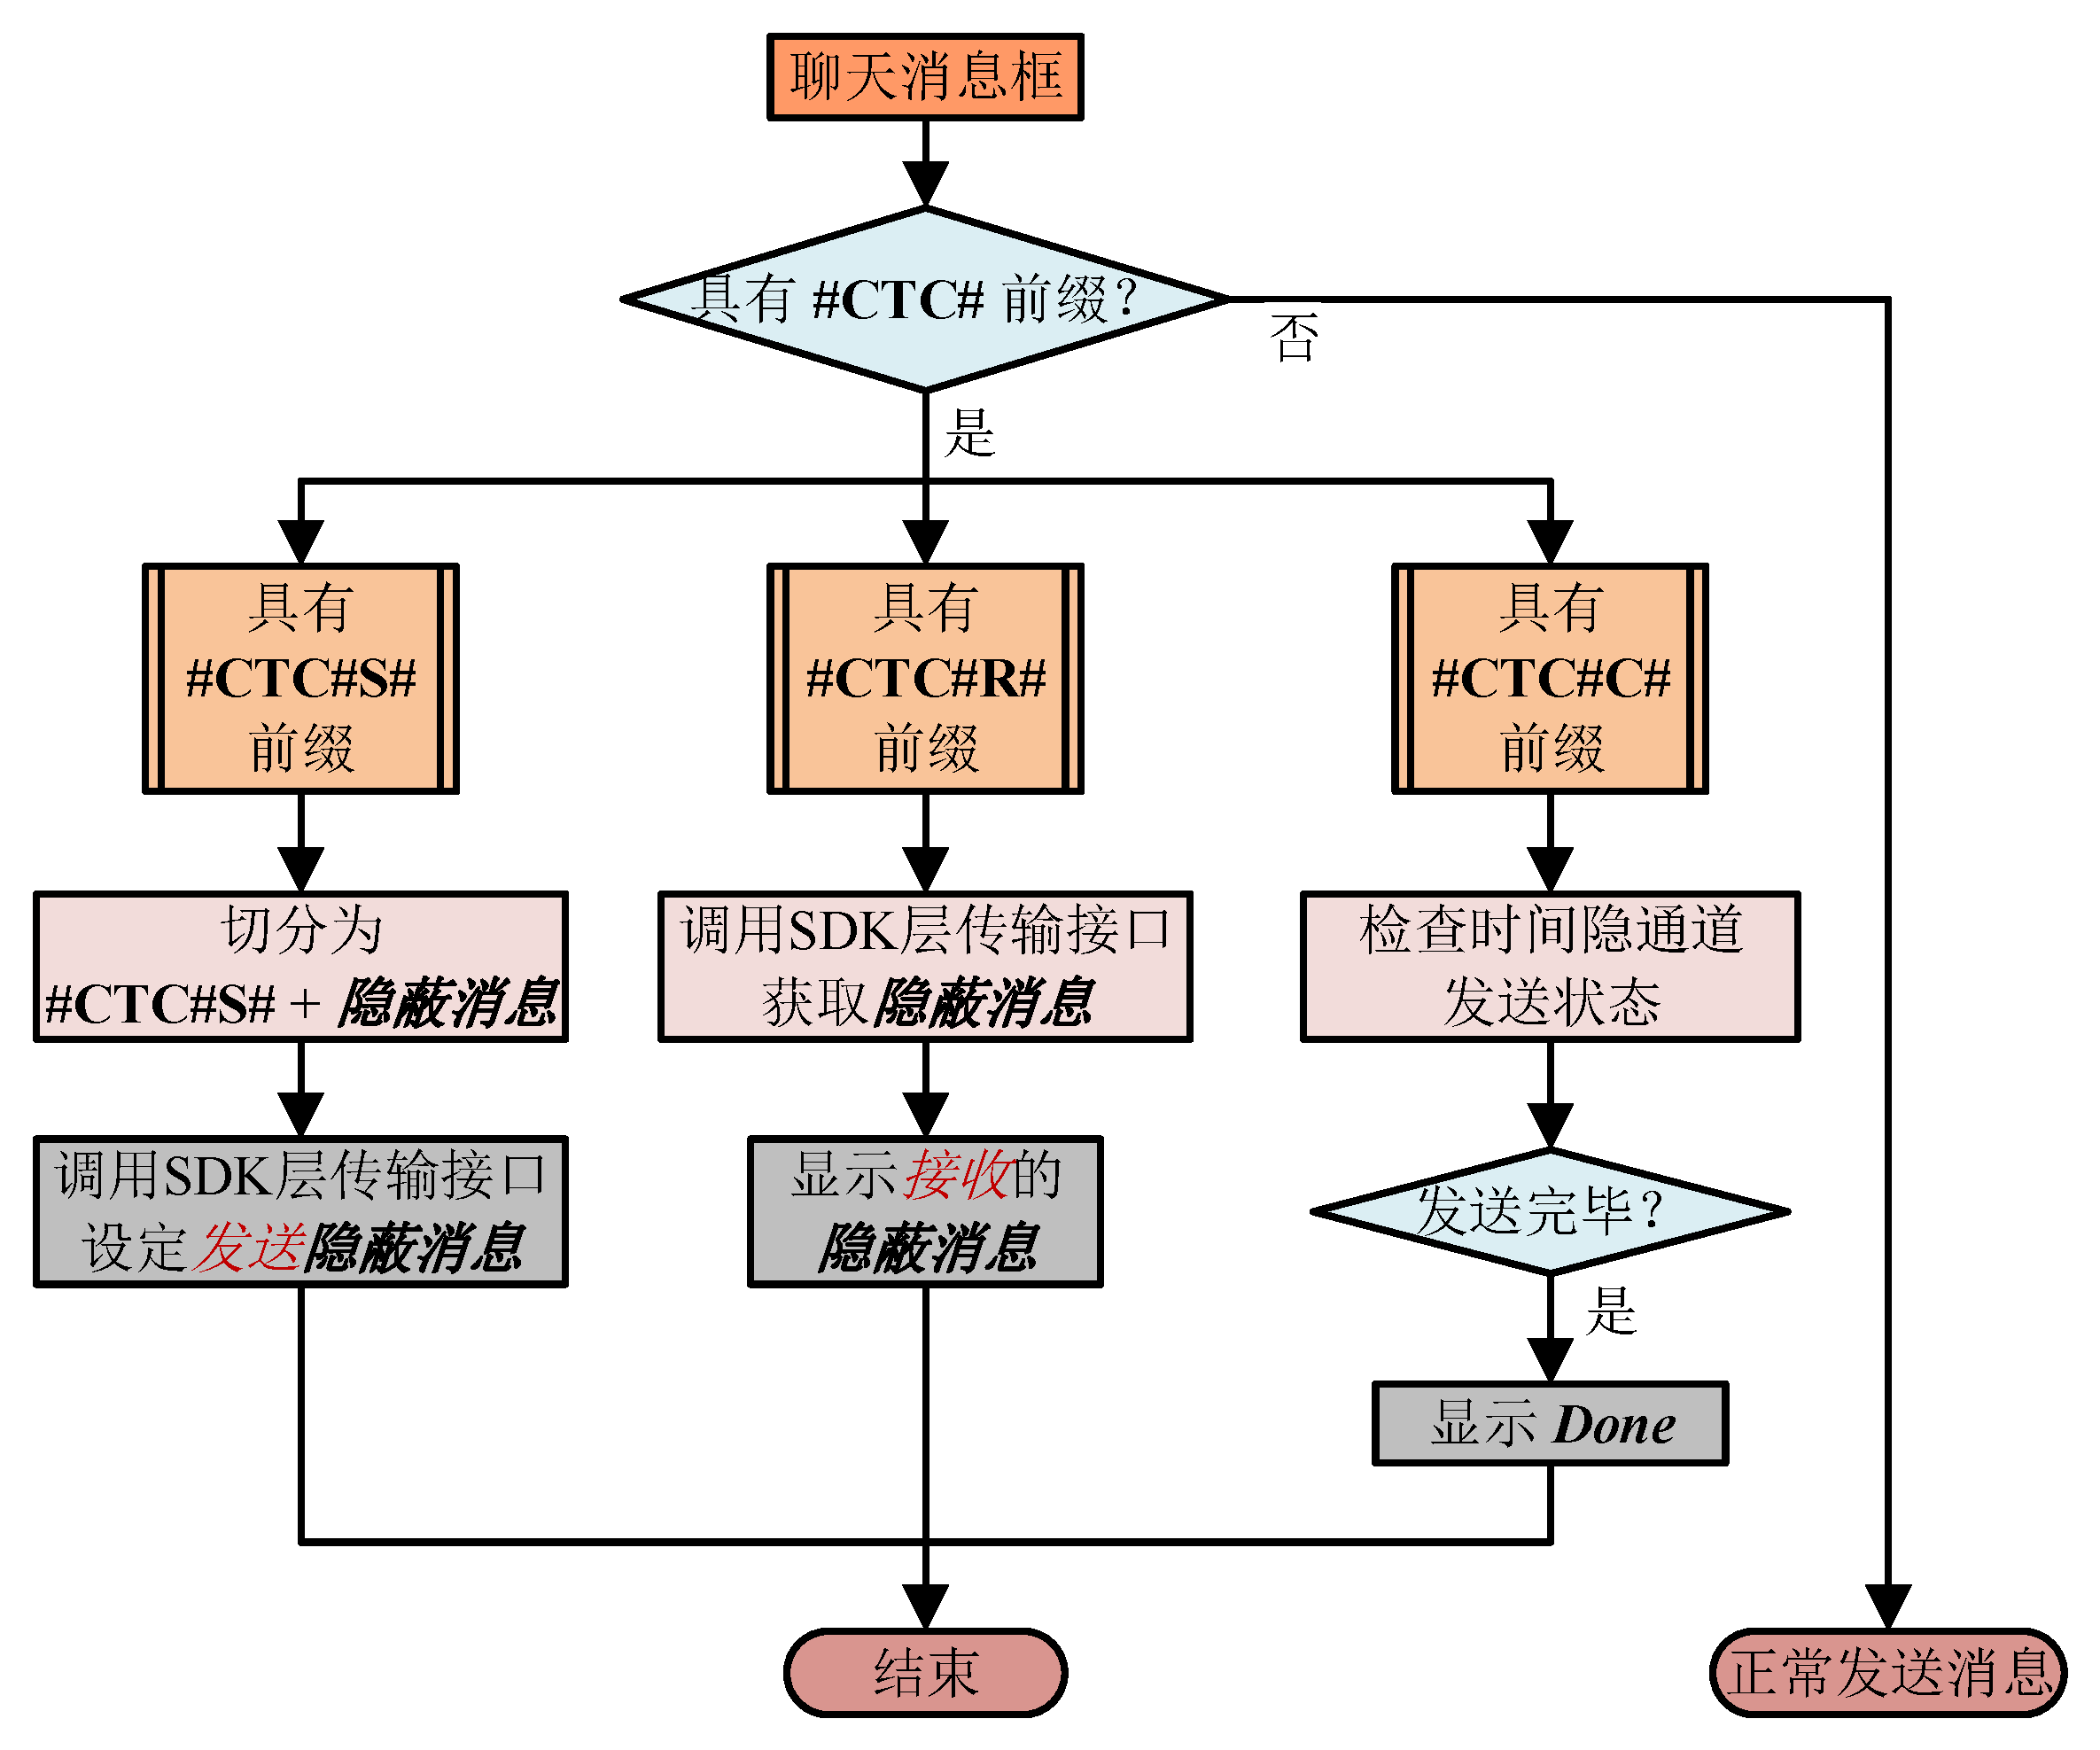
\includegraphics[width=0.75\textwidth]{chapters/chapter6/figures/ui-flow.pdf}
        \caption{原型系统用户界面的控制接口设计}
        \label{fig:6:ui-flow}
    \end{figure}
}

如图\ \nref{fig:6:ui-flow},控制接口为时间隐通道提供了三个控制命令,分别对应发送隐蔽消息、获取隐蔽消息及检查发送状态。三个命令均通过聊天界面输入框触发,前缀‘\texttt{\#CTC\#S\#}’对应发送隐蔽消息,前缀‘\texttt{\#CTC\#R\#}’对应获取隐蔽消息,前缀‘\texttt{\#CTC\#C\#}’对应检查发送状态。当触发隐蔽消息发送时,首先将输入内容进行切分,前缀‘\texttt{\#CTC\#S\#}’后的内容设定为隐蔽消息,然后调用SDK层的隐通道消息接口设定消息内容。当触发隐蔽消息接收时,调用SDK层的隐通道消息接口,获取当前已经接收的隐蔽消息,并在输入框中进行显示。当触发发送状态检查时,调用SDK层的隐通道消息接口,判断当前的隐蔽消息是否传输完毕,如传输完毕则显示‘\texttt{Done}’确认。

\subsection{oRTP传输控制设计}
\label{chap:linphone:designation:ortp}

\insertFigure{
	\begin{figure}[htb]
		\centering
        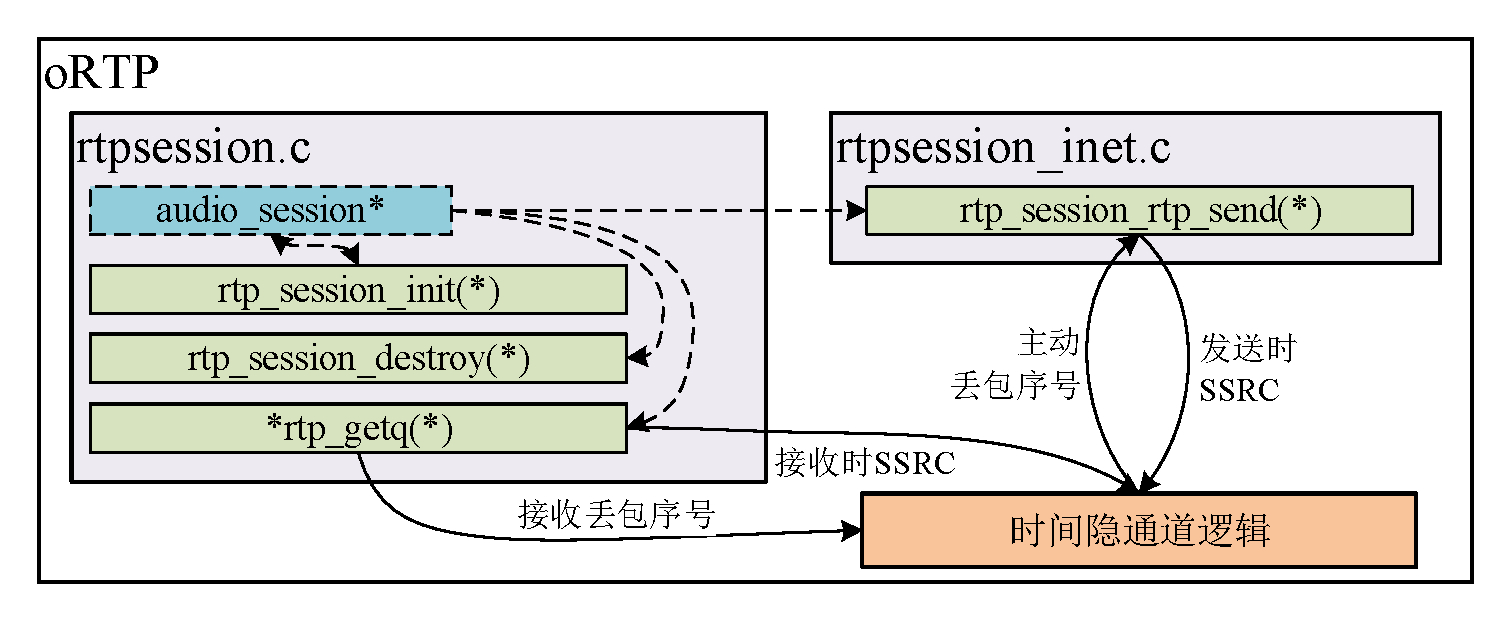
\includegraphics[width=0.9\textwidth]{chapters/chapter6/figures/ortp-flow.pdf}
        \caption{oRTP中时间隐通道的数据流}
        \label{fig:6:ortp-flow}
    \end{figure}
}

oRTP层添加的功能主要包含三部分,分别为数据流识别、丢包序号监听以及主动丢包控制。其中,数据流识别与丢包序号监听位于\texttt{rtpsession.c}文件,主动丢包控制位于\texttt{rtpsession\_inet.c}文件。数据流识别部分通过指针\texttt{audio\_session}记录语音会话的指针,当执行\texttt{rtp\_session\_init}初始化时进行设定,通话结束执行\texttt{rtp\_session\_destroy}时进行清理。丢包序号监听位于\texttt{rtp\_getq}函数内部,通过\texttt{audio\_session}识别语音数据流后,由数据包接收队列判断未接收到的序号,并将结果传输到时间隐通道逻辑组件。主动丢包控制位于\texttt{rtp\_session\_rtp\_send}函数内部,该函数由发送队列中取出数据包后,交付网络组件传输。通过判断数据包序号是否为丢弃目标,执行传输或销毁操作。此外,接收与发送过程中,RTP包头中的SSRC字段被反馈到时间隐通道逻辑组件,用于调制解调过程的随机化处理。

\subsection{消息传输机制设计}
\label{chap:linphone:designation:data}

\insertFigure{
	\begin{figure}[htbp]
		\centering
        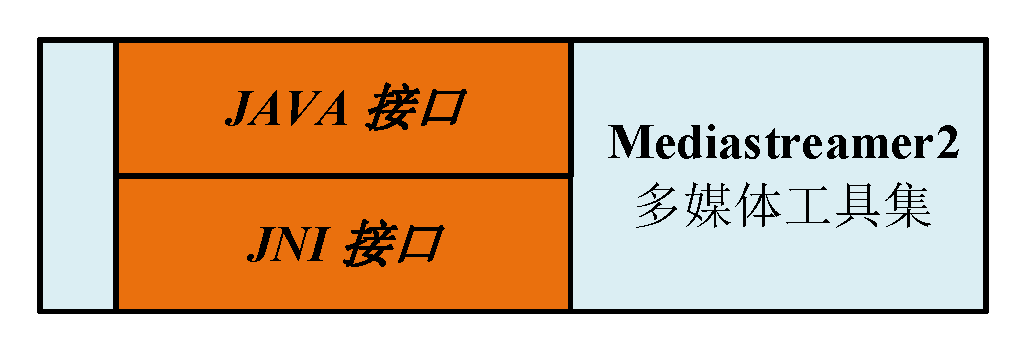
\includegraphics[width=0.4\textwidth]{chapters/chapter6/figures/data-flow.pdf}
        \caption{原型系统消息传输接口的构成结构}
        \label{fig:6:data-flow}
    \end{figure}
}

如图\ \nref{fig:6:data-flow},Mediastreamer2中时间隐通道的消息传输接口由两部分组成。接口包含Linphone SDK提供给UI层的JAVA接口,以及面向oRTP层中时间隐通道逻辑组件的JNI调用。根据Linphone软件架构设计,Linphone SDK与UI层通过JAVA接口进行数据传输,从而实现内存隔离及内部数据保护。因此,原型系统隐通道控制接口与隐通道执行组件的交互,按照相同的模式添加各部分接口。同时在数据类型方面,实现C数据类型与JAVA数据类型的相互转换,从而实现消息传输。

\subsection{调制解调方法设计}
\label{chap:linphone:designation:modulation}

本文中提出了两种时间隐通道构建方法,二者均通过参数$L_{Codeword}$控制主动丢包密度。Linphone与VoLTE在网络环境方面存在差异,因此原型系统采用了简化的调制解调方法。由于Linphone支持NAT转换,完成NAT转换前存在链接切换,此时传输可靠性较差。因此,时间隐通道跳过前200个数据包以获取稳定的传输,按照语音数据包{50\ pkts/s}的发送速率,200个数据包对应{4\ s}左右的通话时间。

\insertFigure{
	\begin{figure}[htb]
		\centering
        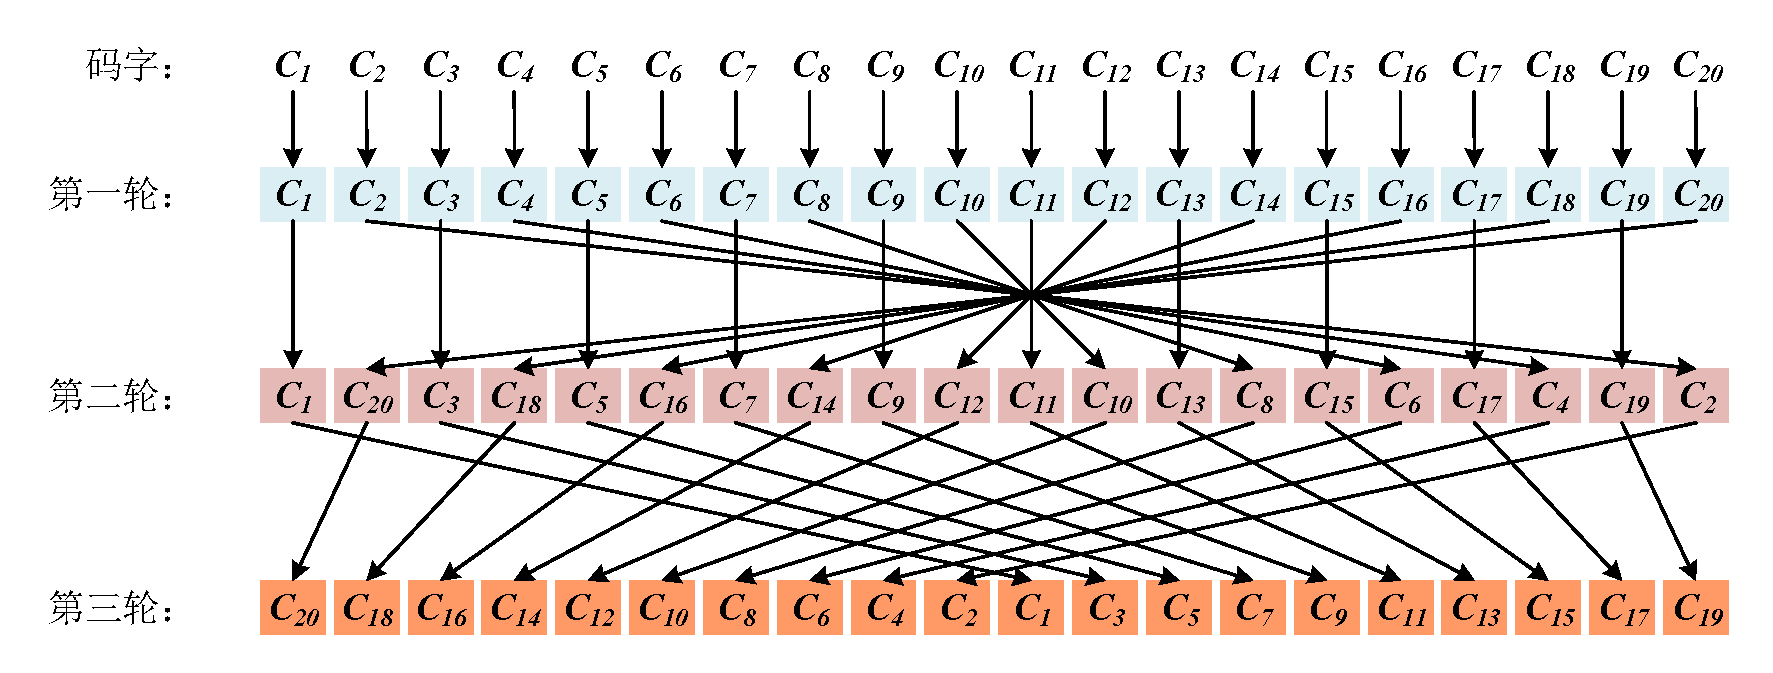
\includegraphics[width=0.95\textwidth]{chapters/chapter6/figures/codeword-cycle.pdf}
        \caption{原型系统中码字发送轮次及顺序}
        \label{fig:6:codeword-cycle}
    \end{figure}
}

如图\ \nref{fig:6:codeword-cycle},以20个码字为单位组构建传输循环,每个码字都会被重复发送三次,每轮按照不同的组织顺序。时间隐通道接收方将数据包序号转换为码字后,将三个轮次的结果取交集,即可去除网络噪声干扰。如图\ \nref{fig:6:ortp-flow},RTP包头中的SSRC反馈到时间隐通道逻辑组件,以SSRC为随机数种子迭代伪随机数生成器,实现传输过程随机化。

\subsection{时间隐通道工作流程}
\label{chap:linphone:designation:workflow}

\insertFigure{
	\begin{figure}[htb]
		\centering
        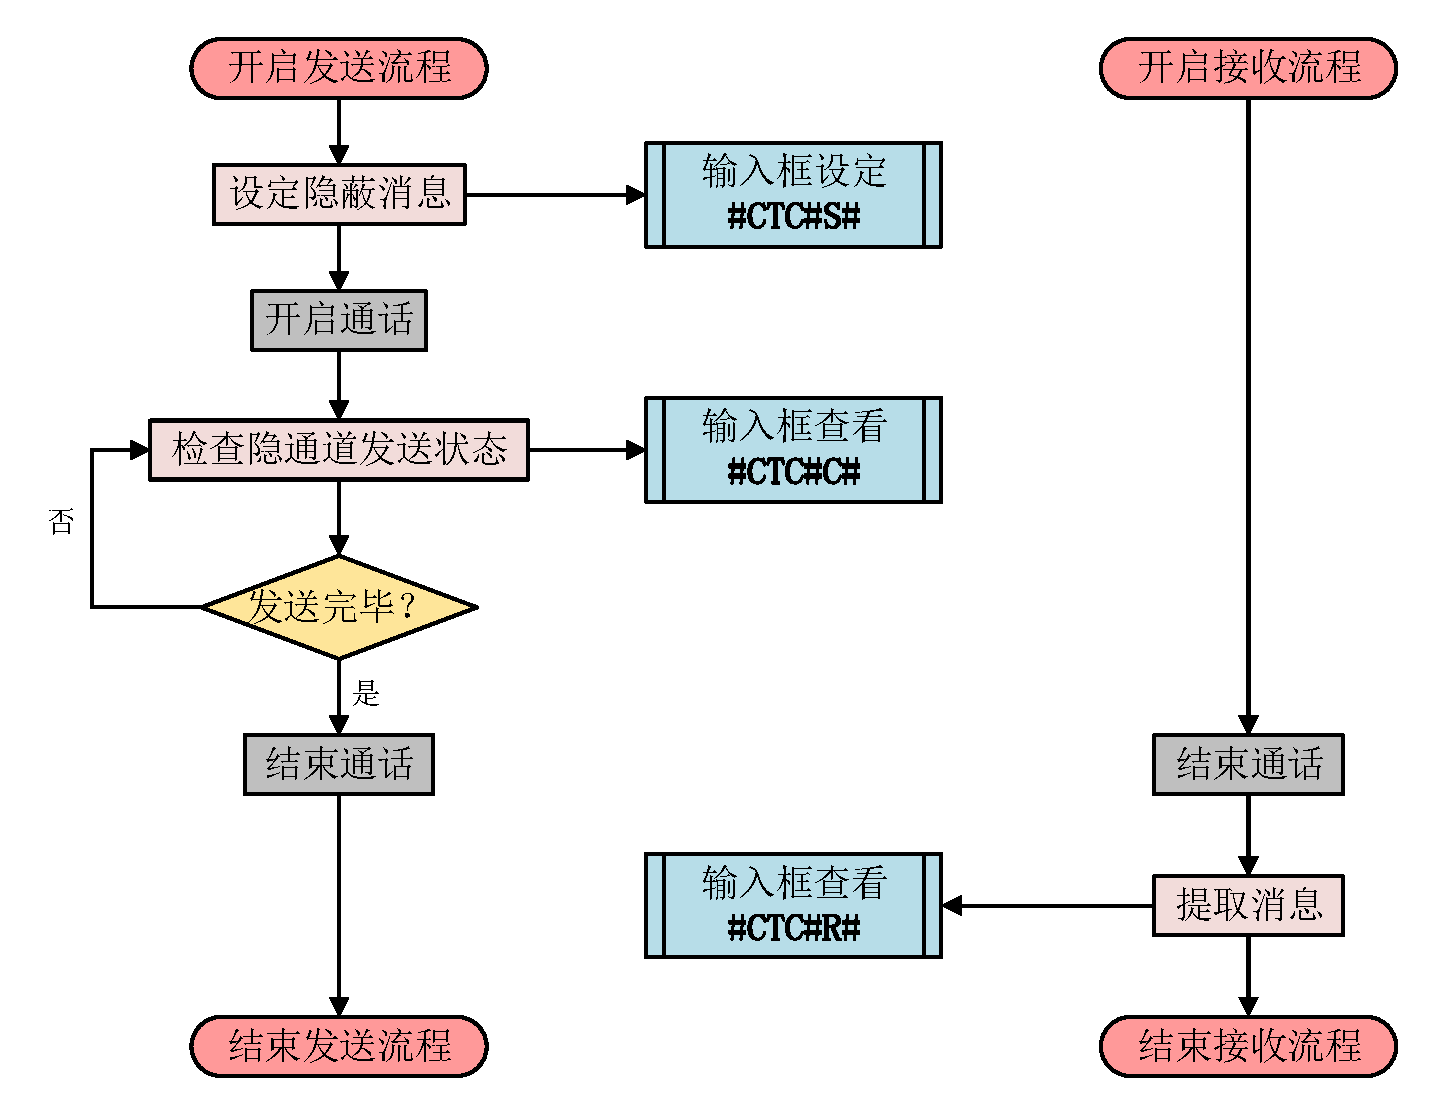
\includegraphics[width=0.7\textwidth]{chapters/chapter6/figures/call-ctc.pdf}
        \caption{Linphone通话与时间隐通道工作流程}
        \label{fig:6:call-ctc}
    \end{figure}
}

如图\ \nref{fig:6:call-ctc},时间隐通道的工作流程与Linphone通话流程密切相关。基于主动丢包的时间隐通道具备双工能力,同时进行发送与接收。发送流程中,首先设置待发送的隐蔽消息,然后开启通话。发送方查看状态确认消息发送完毕后,即可结束通话。接收流程监听数据包序号,然后在通话结束后执行解调流程,接收方即可查看消息内容。在双工模式下,通话双方既是发送方又是接收方,具备信息交换能力。